\section{Roboterregelung \robo{155}{7}}
\begin{minipage}{0.5\linewidth}
    \textbf{Regelung}
    \begin{itemize}
        \item Lageregelung
        \begin{itemize}
            \item Unabhängig von den Bearbeitungkräften/Momenten
            \item Im Gelenkraum ->PID oder Modelbasiert
            \item im kartesischen Raum ->Gelenkbasiert über kinematik oder invers Jacobi
        \end{itemize}
        \item Kraftregelung
        \begin{itemize}
            \item definiert Kräfte/Drehmomente auf die Arbeitsumgebung
        \end{itemize}
        \begin{itemize}
            \item Mischform zwischen Lage und Kraftregelung
        \end{itemize}
        \item hybride Regelung
        \item Interne und externe Roboterregelung
        \item Lineare Regelung
        \item Modelbasierte Regelung
        \item Adaptive Regelung
    \end{itemize}
\end{minipage}
\begin{minipage}{0.5\linewidth}
    \textbf{Steurung}
    \begin{itemize}
        \item Struktur und Komponenten
        \item Ausführungsbeispielö
        \begin{itemize}
            \item ABB, KUKA, Stäuble
        \end{itemize}
    \end{itemize}
%\end{minipage}
%\begin{minipage}{0.5\linewidth}
\end{minipage}
\textbf{Regelung Infofluss}\newline
    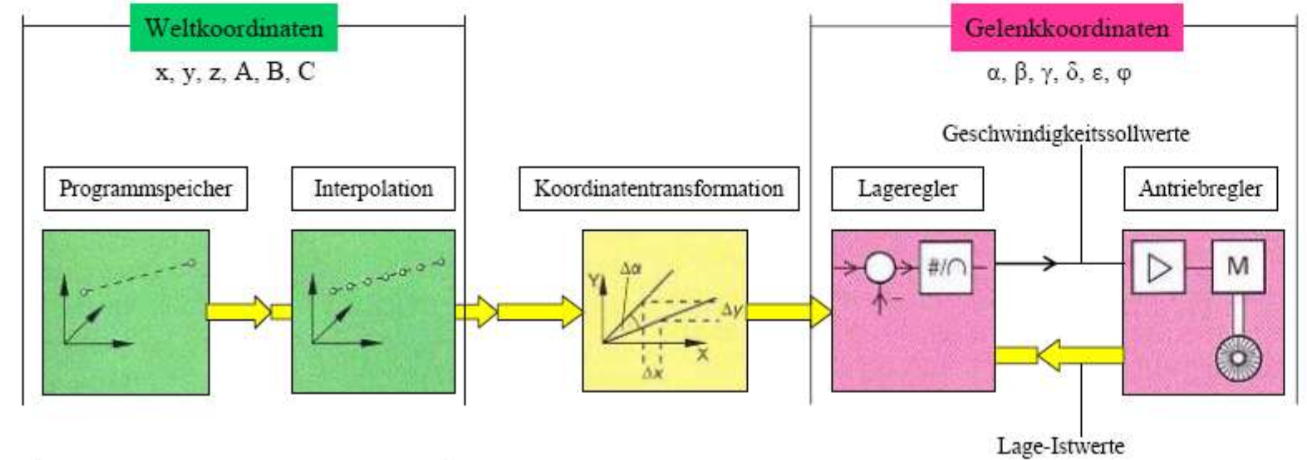
\includegraphics[width=\linewidth]{./bilder/RegelungInfofluss}
%\end{minipage}

\begin{minipage}{0.5\linewidth}
    \subsection{Kartesische Lageregelung}
    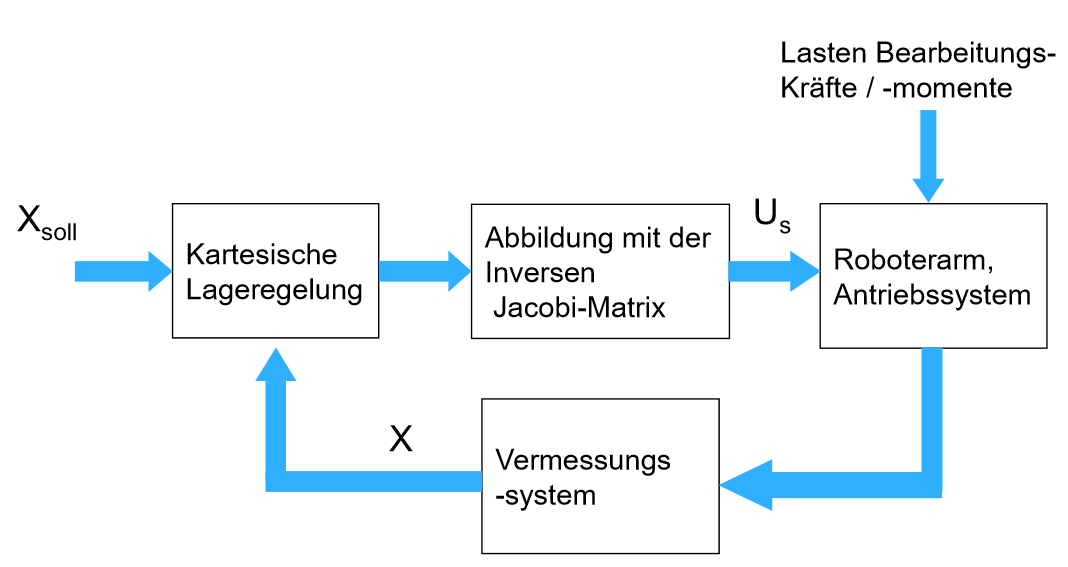
\includegraphics[width=\linewidth]{./bilder/KartLageRegelung}
\end{minipage}
\begin{minipage}{0.5\linewidth}
    \subsection{Interne/ Externe Regelung}
    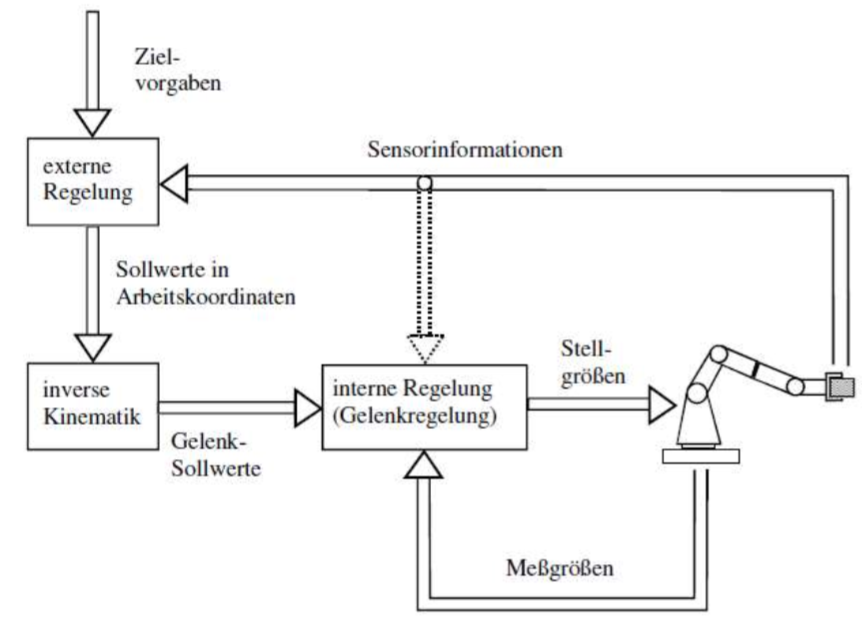
\includegraphics[width=0.8\linewidth]{./bilder/InternExternRegelung}
\end{minipage}
\begin{minipage}{0.5\linewidth}
    \subsection{Kraftregelung}
    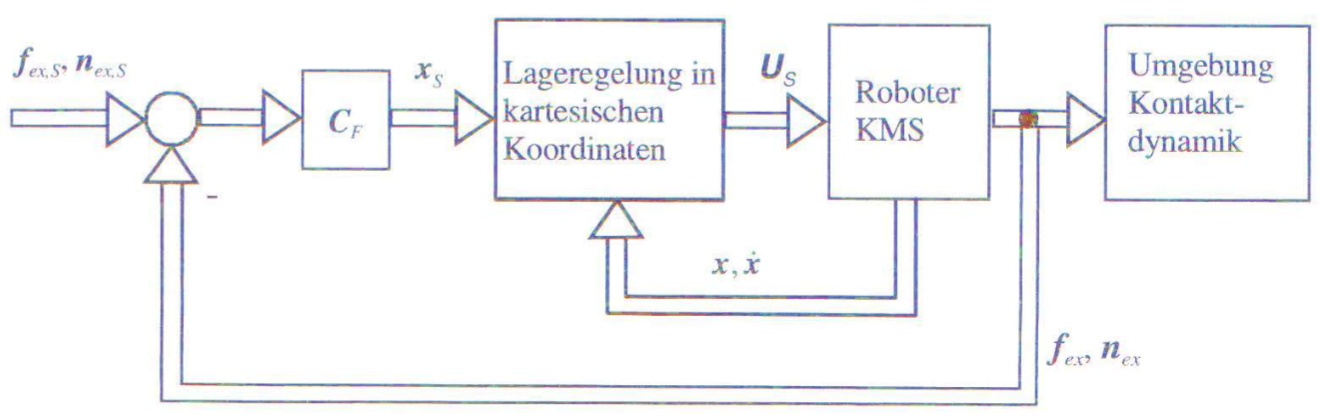
\includegraphics[width=\linewidth]{./bilder/KraftRegelung}
\end{minipage}
\begin{minipage}{0.5\linewidth}
    \subsection{Linearegelung}
    \vspace{-1cm}
    \[ \tau_{FB}=K_p\cdot e + K_d\cdot \dot{e} \]
    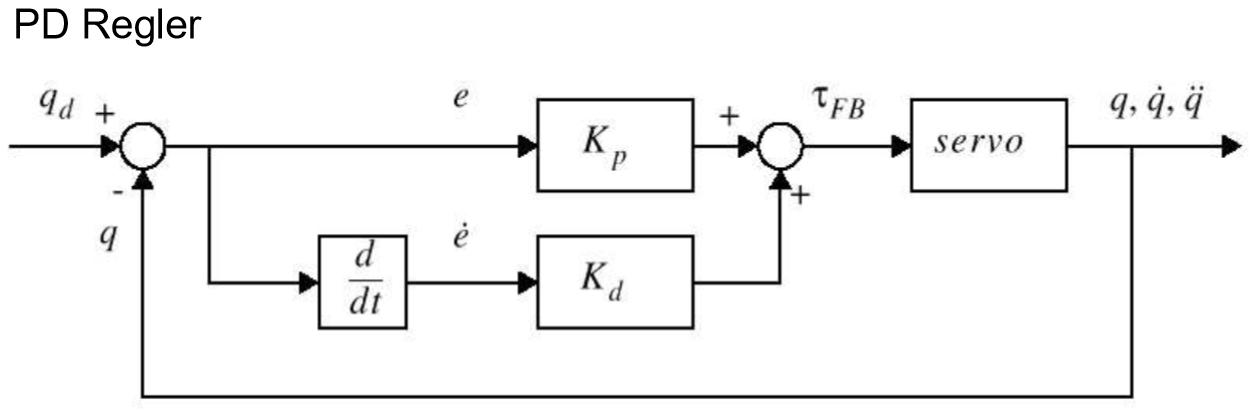
\includegraphics[width=\linewidth]{./bilder/PDRegler}
\end{minipage}
\clearpage

\begin{minipage}{0.5\linewidth}
\subsection{Dynamische Gleichung}
    \[   \tau = M(q)\cdot \ddot{q}+ V(q,\dot{q})+G(q) \]
    Q = verallgemeinerte Kräfte\newline
    M = konfigurationsabhängige Massenmatrix\newline
    V = Vektor nichtlinerer Terme\newline
    \quad (Centripetal und Coriolis-Beschleunigung)\newline
    G = Vektor mit Gravitationsterme
\end{minipage}
\begin{minipage}{0.5\linewidth}
    \subsection{Vorsteuerung}
    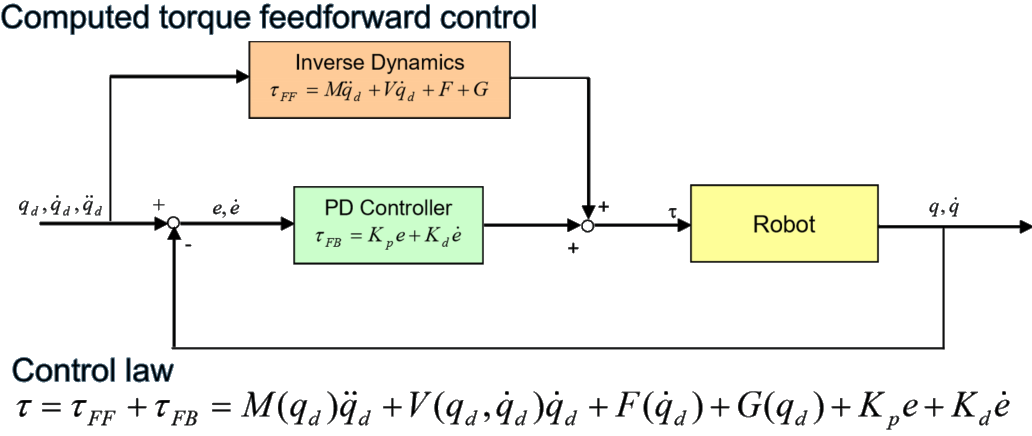
\includegraphics[width=\linewidth]{./bilder/Vorsteuerung}
\end{minipage}
\begin{minipage}{0.5\linewidth}
    \subsection{Drehmomentkontrolle}
    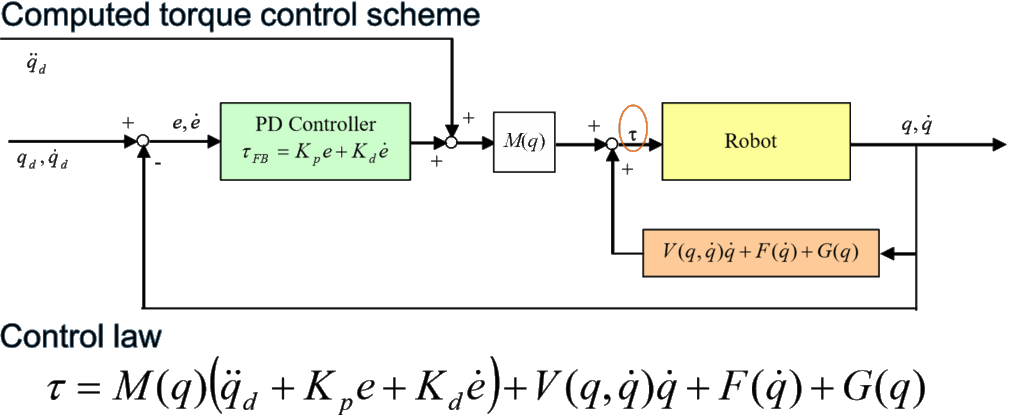
\includegraphics[width=\linewidth]{./bilder/RegMod2}
\end{minipage}
\begin{minipage}{0.5\linewidth}
    \subsection{Nichtlienare Drehmomentkontrolle}
    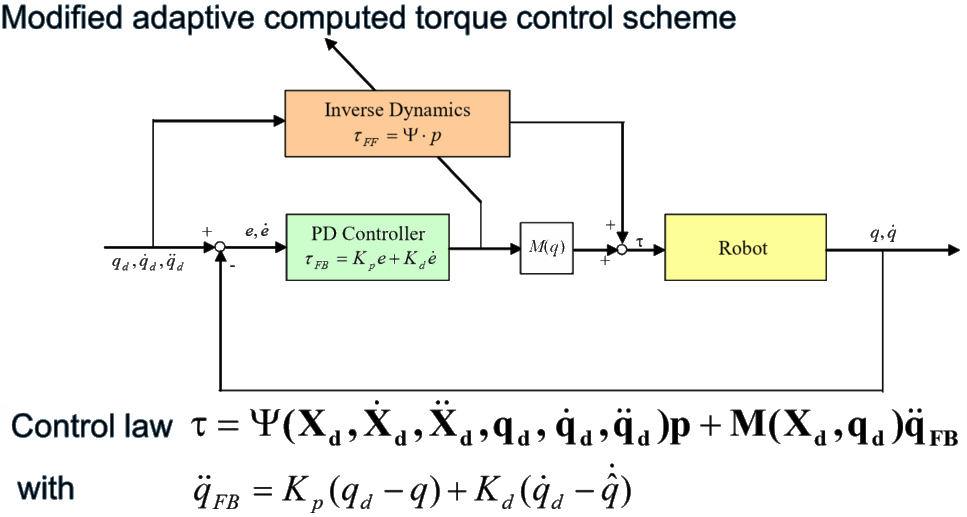
\includegraphics[width=\linewidth]{./bilder/RegModNL}
\end{minipage}

\begin{minipage}[t]{1\linewidth}
    \subsection{Regelung Delta Roboter}
    \raisebox{1\height}{
    \begin{minipage}{0.3\linewidth}
    \begin{itemize}
        \item[]\textbf{Spezifikationen:}
        \item Widerholgenauigkeit v2$\mu$m
        \item Kurze Zykluszeit $\approx$ 3Zyklen/s
    \end{itemize}
\end{minipage}}
    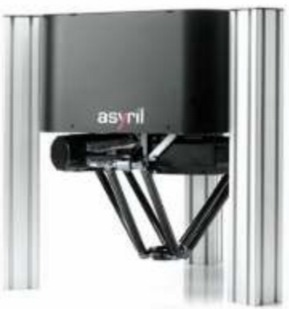
\includegraphics[width=0.17\linewidth]{./bilder/DeltaRob}
    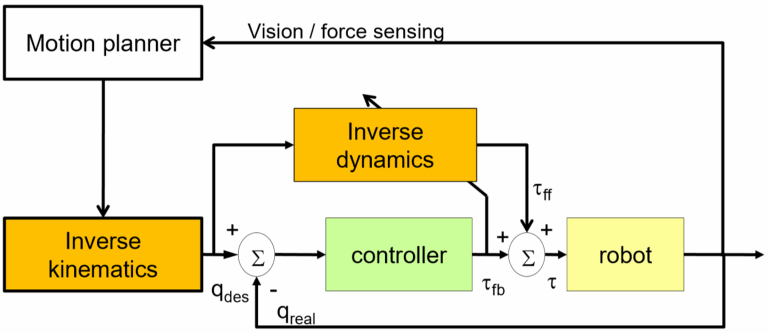
\includegraphics[width=0.5\linewidth]{./bilder/DeltaRobReg}
\end{minipage}
\begin{minipage}{1\linewidth}
    \subsection{Regelung Hexaglide}
    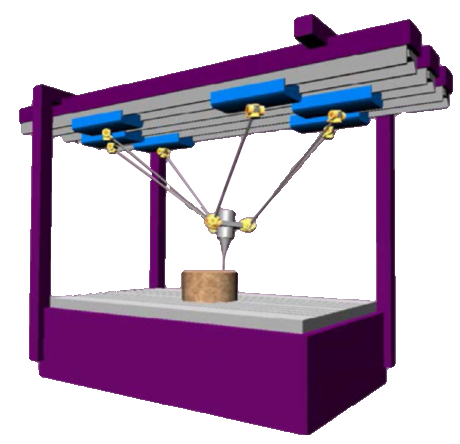
\includegraphics[width=0.2\linewidth]{./bilder/Hexaglide1}
    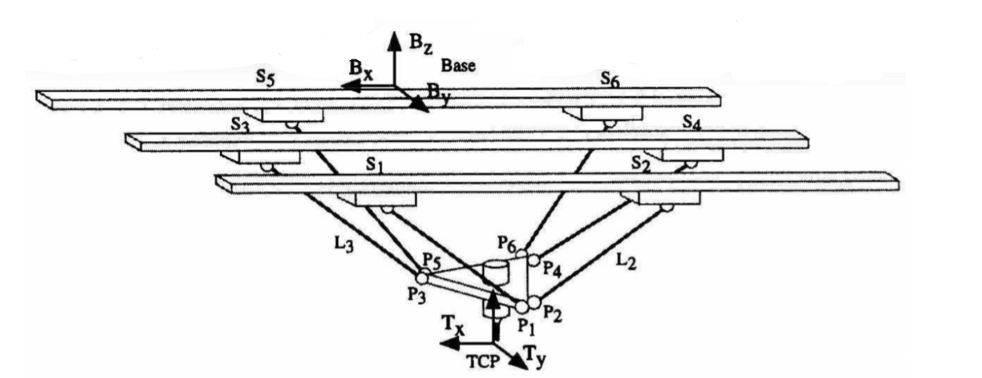
\includegraphics[width=0.3\linewidth]{./bilder/Hexaglide2}
    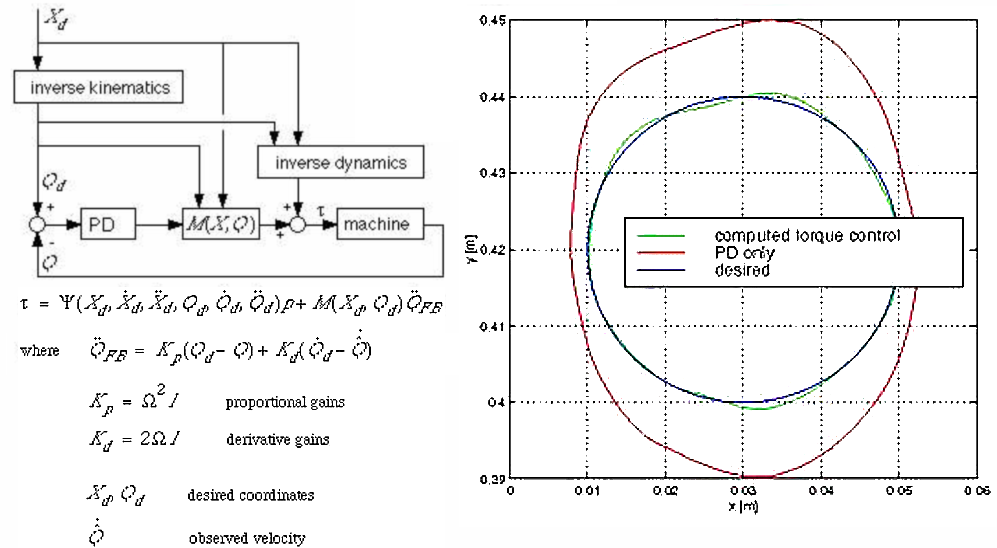
\includegraphics[width=0.5\linewidth]{./bilder/HexaglideReg}
\end{minipage}
\begin{minipage}{0.5\linewidth}
    \subsection{Steuerung ABB}
    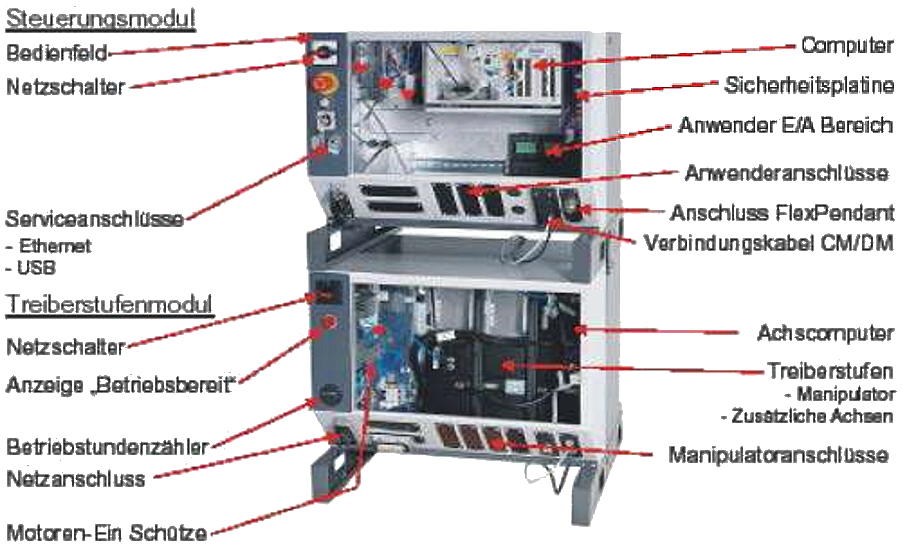
\includegraphics[width=\linewidth]{./bilder/SteuerungABB}
\end{minipage}
\begin{minipage}{0.5\linewidth}
    \subsection{Steuerung Stäubli}
    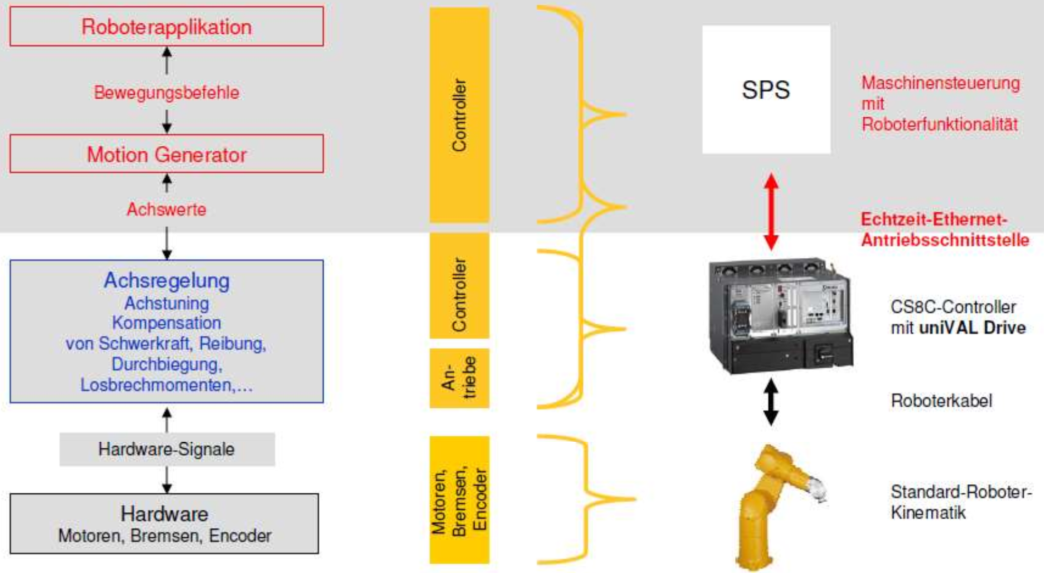
\includegraphics[width=\linewidth]{./bilder/SteuerungStauebli}
\end{minipage}